\documentclass[fleqn]{article}
\usepackage{graphicx}

\title{EE214A Design Project}
\author{Jay Smith}
\date{\today}

\begin{document}
\raggedright
\maketitle
\begin{flushleft}

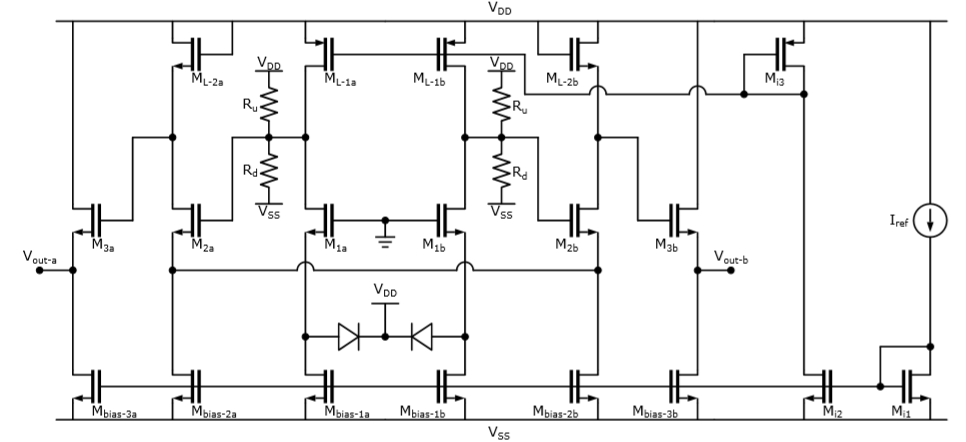
\includegraphics[scale=0.6]{circuit_architecture}

\large{The amplifier under evaluation has 3 stages: 
Common Gate (CG), Common Source (CS), and Common Drain (CD).  In order to analyze, the circuit is broken down into its 3 stages and key parameters are summarized.}\\
\vspace{5mm} 

\begin{tabular}{ | p{6cm} || p{6cm} | }
\hline
Parameter & Spec\\
\hline
Transresistance gain & 42.5k\\
\hline
power consumption & $\leq$2mW\\
\hline
bandwidth & $\geq$75MHz\\
\hline
Output load resistance & 20k\\
\hline
Output load capacitance & 250fF\\
\hline
\end{tabular}
\vspace{10mm}




\newpage
\textbf{Common Gate:}\\
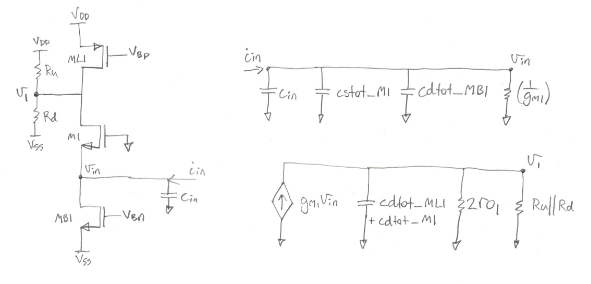
\includegraphics[scale=1.1]{CG_schematic}

\begin{tabular}{ | p{4cm} || p{4cm} | p{4cm} | }
\hline
\multicolumn{3}{ | c | }{ Low Frequency Characteristics }\\
\hline
Transimpedance Gain & R\textsubscript{u} parallel R\textsubscript{d} & \\
\hline
Rin & 1/gm1 & Vov\textsubscript{1}/(2*I\textsubscript{D1})\\
\hline
Rout  & 2*ro\textsubscript{1} & 2/(lambda*I\textsubscript{D1})\\
\hline
\end{tabular}


\newpage
\textbf{Common Source:}\\
The source of the common source stage is referenced to virtual, small-signal ground in the DM half circuit.
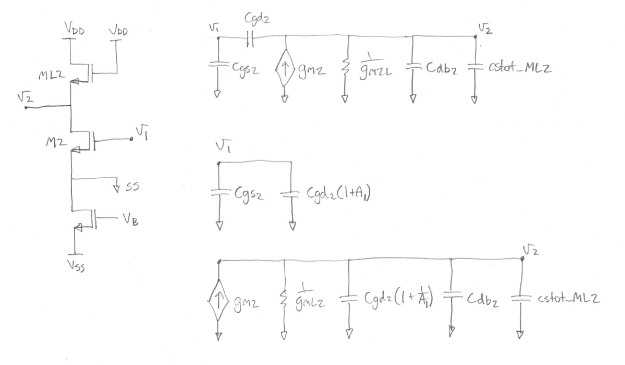
\includegraphics[scale=1.1]{CS_schematic}

\begin{equation}
A_1 = \frac{ gm_{2} }{ gm\textsubscript{L2} }
\end{equation}
\begin{equation}
A_1 = \frac{ \frac{W}{L}_2*Vov_2 }{ \frac{W}{L}_{2L}*Vov_{2L} }
\end{equation}
\begin{equation}
A_1 = \sqrt{ \frac{ \frac{W}{L}_2 }{ \frac{W}{L}_{2L} } }
\end{equation}
\begin{equation}
A_1 = \frac{ Vov_{2L} }{ Vov_{2} }
\end{equation}

\begin{tabular}{ | p{5cm} || p{5cm} | }
\hline
\multicolumn{2}{ | c | }{ Low Frequency Characteristics }\\
\hline
Av & -gm\textsubscript{2}/gm\textsubscript{L2}\\
\hline
Rin & inf\\
\hline
Rout  & 1/gm\textsubscript{L2}\\
\hline
\end{tabular}

\newpage
\textbf{Common Drain:}
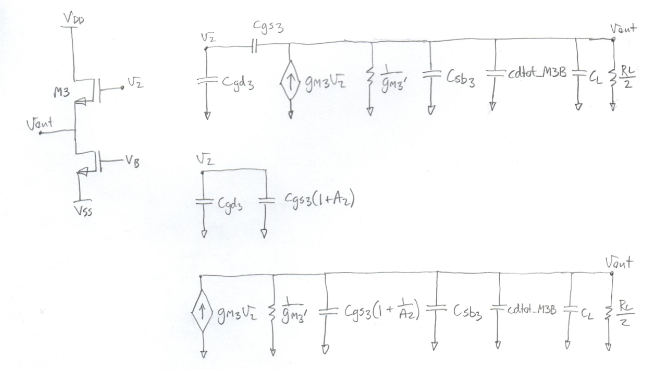
\includegraphics[scale=1.1]{CD_schematic}
\begin{equation}
C_{LDM} = 500fF
\end{equation}
\begin{equation}
R_{LDM} = 10k\Omega
\end{equation}
Assuming R\textsubscript{L}/2 much less than 1/gm\textsubscript{3}
\begin{equation}
A_2 = -g_{m3}*\frac{1}{g_{m3}'}||R_{LDM} \approx -0.84
\end{equation}

\begin{tabular}{ | p{5cm} || p{5cm} | }
\hline
\multicolumn{2}{ | c | }{ Low Frequency Characteristics }\\
\hline
Av & approx. 0.84\\
\hline
Rin & inf\\
\hline
Rout  & 1/gm\textsubscript{3}'\\
\hline
\end{tabular}



\newpage
\textbf{TIA amp:}\\
\vspace{5mm}
Small-Signal Model
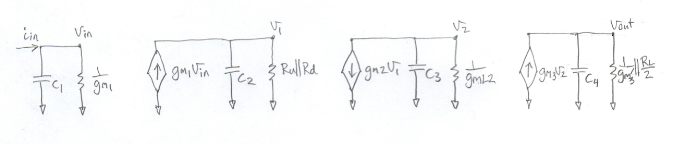
\includegraphics[scale=1]{full_small_signal}
Low Frequency Transimpedance Gain:
\begin{equation}
\frac{v_{out}}{i_{in}} = (R_u || R_d)*(-\frac{ gm_{2} }{ gm\textsubscript{L2} })*0.84
\end{equation}

BW
\begin{equation}
C_{LDM} = 500fF
\end{equation}
\begin{equation}
R_{LDM} = 10k\Omega
\end{equation}

\begin{equation}
C_1 = 100fF + cstot\_M1 + cdtot\_MB1
\end{equation}
\begin{equation}
C_2 = cdtot\_ML1 + cdtot\_M1 +  C_{gs2} + (1 + A_1)*C_{gd2} 
\end{equation}
\begin{equation}
C_3 = (1 + 1/A_1)*C_{gd2} + C_{db2} + cstot\_ML2 + C_{gd3} + (1 + A_2)*C_{gs3}
\end{equation}
\begin{equation}
C_4 = (1 + 1/A_2)*C_{gs3} + C_{sb3} + cdtot\_M3B + 500fF
\end{equation}

\begin{equation}
A_1 = \frac{ gm_{2} }{ gm\textsubscript{L2} }
\end{equation}
\begin{equation}
A_1 = \frac{ \frac{W}{L}_2*Vov_2 }{ \frac{W}{L}_{2L}*Vov_{2L} }
\end{equation}
\begin{equation}
A_1 = \sqrt{ \frac{ \frac{W}{L}_2 }{ \frac{W}{L}_{2L} } }
\end{equation}
\begin{equation}
A_1 = \frac{ Vov_{2L} }{ Vov_{2} }
\end{equation}
\begin{equation}
A_2 = -g_{m3}*\frac{1}{g_{m3}'}||R_{LDM} \approx -0.84
\end{equation}


ZVTC bandwidth (conservative approximation)
\begin{equation}
b1 = \frac{1}{g_{m1}}*C_1 + (R_u || R_d)*C_2 + gm_{L2}*C_3 + (gm_3'||R_L/2)*C_4
\end{equation}


\end{flushleft}
\end{document}